A proof of the dummy lemma relies on creating a simulator \Sim for an arbitrary adversary given \DS.
Recall from the original discussion in Section~\ref{sec:dummy} that the intuition behind the Dummy Lemma can be seen from the basic definition of emulation.

Consider UC emulation with respect to the dummy adversary. The emulation definition quantifies over all environments. 
This includes an environment that runs any arbitrary real-world adversary \A, for the protocol, internally, and \Z forwards the outputs from the adversary to the dummy adversary and dummy simulator in the execution.
Consider the modified execution where \A is run in the real execution instead of internally: it is the adversary in the real world and it is run as part of the simulator in the ideal world.
The ideal world simulator runs \A and the dummy sim internally and passes input from \Z to \A and output from \A to \DS.
Moving ITMs from inside \Z to the real world is a common pattern in UC proofs and is used in the composition proof as well.
We depict the intuition in Figure~\ref{fig:dummylemmas}.

\begin{figure}
	\begin{subfigure}[t]{0.45\textwidth}
	\centering
	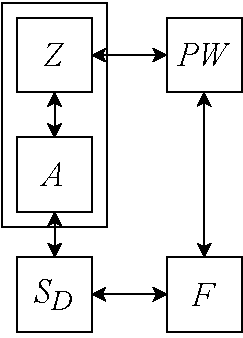
\includegraphics[scale=0.5]{figures/dummylemma_pre.pdf}
	\caption{The ideal world with an environment running an arbitrary \A internally.}
	\label{fig:dummy_pre}
	\end{subfigure}
	\hspace{2mm}
	\begin{subfigure}[t]{0.45\textwidth}
	\centering
	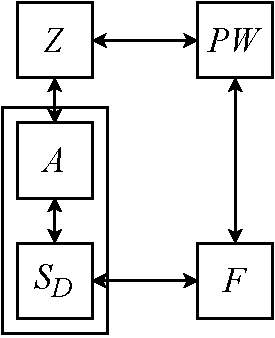
\includegraphics[scale=0.5]{figures/dummylemma_post.pdf}
	\caption{Moving \A into the adversary in the real and ideal world equates to an equivalent execution. Inputs and outputs to \DS are unchanged as are inputs to protocol parties and the functionality. Therefore, we expect the behavior of the execution to be unchanged.}
	\label{fig:dummy_post}
	\end{subfigure}
	\caption{Graphical illustration of the intuition behind the Dummy Lemma as relying on dummy simulation to introduce an adversary.}
	\label{fig:dummylemmas}
\end{figure}


We restate the Dummy Lemma here:
\begin{theorem}[Dummy Lemma]\label{thm:dummy}
If \ $\exists \DS$ s.t. $ \DA, \DS \vdash \F_2 \xrightarrow{\pi} \F_1$ then $\forall \A \ \exists \Sim_\A$ s.t. $\Sim_{\A} \vdash  \F_2 \xrightarrow{\pi} \F_1)$ 
\end{theorem}

\begin{proof}
The constructed simulator $\Sim_\A$ runs \A and \DS internally.
$\Sim_\A$ sandboxes the two simulators using our virtual tokens construction.
The construction simulator is straightforward, and we provide sample snippets of code from the simulator.
The adversaries \A and \DS expect to receive input from \Z through communicator.

Input from \Z is passed to \A:
\begin{lstlisting}[basicstyle=\footnotesize\BeraMonottFamily, frame=single,  mathescape]
msg = $\tb{recv}$ $\$$z_to_a ;
case msg (
  Z2A2P(pid, msg) =>
    $\tb{get}$ $\$$z_to_a {z2an : K} ;
    $\tm{withdrawTokens}$ f K K1 z2an;
    $\$$a_z2a.SEND ;
    $\nsend$ $\$$a_z2a Z2A2P(pid, msg) ;
    $\npay$ {z2an : K1} $\$$a_z2a ;
    $\$$ch <- sim_a_a2p <- ... 
  Z2A2F(msg) =>
    $\tb{get}$ $\$$z_to_a {z2an : K} ;
    $\tm{withdrawTokens}$ f K K1 z2an ;
    $\$$a_z2a.SEND ;
    $\nsend$ $\$$a_z2a Z2A2F(msg) ;
    $\npay$ {z2an : K1} $\$$a_z2a ;
    $\$$ch <- sim_a_a2f <- ... ;
\end{lstlisting}
\end{proof}
It is worth noting that in NomosUC existing processes can be run directly in a sandbox just be using a virtual token.
This is different from the UC notion of the universal turing machine where other ITMs are first encoded as data.

Output from \A to the \partywrapper or \F is passed as \inline{Z2A2P} or \inline{Z2A2F} input to \DS using the same token type \inline{K1}.
Output from \DS is forward along to the outside world as adversary input to the dummy parties and the ideal functionality:
\begin{lstlisting}[basicstyle=\footnotesize\BeraMonottFamily, frame=single, mathescape]
msg = $\nrecv$ $\$$ds_a2p ;
$\nget$ $\$$ds_a2p {a2pn : K1} ;
$\$$a_to_pw.SEND ;
$\nsend$ $\$$a_to_pw msg ;
$\npay$ $\$$a_to_pw {a2fpn : K} ;
\end{lstlisting}
